\documentclass{article}
\usepackage[utf8]{inputenc}
\usepackage{pgfplots}
\usepackage[utf8]{inputenc}
\usepackage[shortlabels]{enumitem}
\usepackage{amsmath}
\usepackage{amssymb}
\usepackage{gensymb}
\usepackage{geometry}
\usepackage{listings}
\usepackage{xcolor}
\usepackage{pgfplots}
\usepackage{pgfplotstable}
\usepgfplotslibrary{statistics}
\usepgfplotslibrary{fillbetween}
\pgfplotsset{compat=1.7}
\usepackage{tikz}
\geometry{
 a4paper,
 total={170mm,257mm},
 left=20mm,
 top=20mm,
}

\title{Statistics Unit}
\author{Andy Yan}
\date{September 2023}

\begin{document}

\maketitle

\section{Data Analysis Grouped Data}

\large\textbf{Raw Data:}\\
35.6,  39.3,  39.8,  40.8,  43.9,  45.7,  45.9,  47.5,  48.6,  49.2,  52.6,  55.4,  56.4,  57.4,  58.1,  58.8,  60.0,  62.2,  63.7,  64.2,  64.5,  64.9,  66.9,  68.3,  68.8,  70.1,  70.7,  73.3\\

\normalsize
\noindent
\textbf{Basic Terms:}\\
Raw Data: The unprocessed information collected for a study\\
Continuous Variable: Can have any value within the range (Ex: Volume, Weight)\\
Discrete Variable: Can have only separate values, mostly integers (\# of people)\\\\
\textbf{Grouped Data}\\
Grouped Data is organized with intervals and the frequency within the intervals.

\begin{center}
\def\arraystretch{1}
\begin{tabular}{| c | c | c | c | c |} 
\hline
\multicolumn{5}{|c|}{Cumulative Relative Frequency Table} \\
 \hline
   Class Interval & Frequency & Cumulative Frequency & Relative Frequency & Cumulative Relative Frequency\\
 \hline
35.6 - 41.1 & 4 & 4 & 0.1429 & 0.1429\\
 \hline
42.1 - 47.6	& 4 & 8 & 0.1429 & 0.2857\\
 \hline
48.6 - 54.1	& 3 & 11 & 0.1070 & 0.3929\\
 \hline
55.1 - 60.6	& 6 & 17 & 0.2143 & 0.6071\\
 \hline
61.6 - 67.1	& 6 & 23 & 0.2143 & 0.8217\\
 \hline
 68.1 - 73.6	& 5 & 28 & 0.1786 & 1\\
  \hline
\end{tabular}
\end{center}

Number of Values \(\textbf{n}\)\\
\# of class intervals \(\textbf{c} = \lceil 1 + 3.222\log(n)\rceil\)\\
Interval Size \(\textbf{i} = \lceil \frac{\textbf{Max } - \textbf{ Min}}{c}\rceil\)\\\\
Frequency (F) : \# of occurrences for a variable\\
Cumulative (C) : Totaling \# of\\
Cumulative Frequency (CF) : \(CF_k = F_k + CF_{k-1}\)\\
Relative Frequency (RF) : \(RF = \frac{F}{n}\)\\
Cumulative Relative Frequency (CRF) : \(CRF_k = RF_k + CRF_{k-1}\)

\section{Measures of Spread}
\textbf{Standard Deviation for Population}\\
\[\sigma = \sqrt{\frac{\sum(x_i-\mu)^2}{N}} = \sqrt{\frac{\sum(x_i-\mu)^2}{\sum f_i}} \]
\textbf{Standard Deviation for Sample}\\
\[s = \sqrt{\frac{\sum(x_i-\Bar{x})^2}{N-1}}\]
\textbf{\(Z\)-score}\\
\[Z_i = \frac{x_i-\mu}{\sigma}\]
\section{Percentile}
\Large \textbf{\(P_{PR}\)}\\
\normalsize \(PR\) is the percentage of numbers \(P_{PR}\) is bigger than\\
\textbf{Percentile Rank Ungrouped Data}\\
Central Tendency: Mean Median Mode\\
\begin{minipage}[t]{0.5\textwidth}
\[PR = \frac{b + \frac{1}{2}e}{n} \cdot 100\%\]
\end{minipage}
\begin{minipage}[t]{0.6\textwidth}
\vspace{0.3em}
b: how many values below\\
e: how many equal values
\end{minipage}
\[k = PR \cdot (total + 1) = \textbf{a number greater than PR\% of the data}\]
\[P_{PR} = x_{\lfloor k \rfloor} + (\lceil k \rceil - k) \cdot (x_{\lceil k \rceil} - x_{\lfloor k \rfloor})\]

\noindent
\textbf{Percentile Rank Grouped Data}\\
\(\Bar{x}_i\): middle value for the \(i^{th}\) interval\\
\(f_i\): frequency value for the \(i^{th}\) interval\\
Central Tendency:
\begin{enumerate}
    \item Mode: value of \(\Bar{x}_i\) in the interval with greatest frequency
    \item Median = \(l + (\frac{\frac{n}{2}-cf}{f}) \cdot h\)\\
    To determine the median class, locate which class' cumulative frequency is closest to \(\frac{n}{2}\).
    \begin{itemize}
        \item \(l\) is the lower limit of the median class
        \item \(n\) is the number of observations
        \item \(f\) is the frequency of the median class
        \item \(h\) is the class size
        \item \(cf\) is the cumulative frequency of the class PRECEDING the median class
    \end{itemize}
    \item Mean = \(\frac{\displaystyle \sum_{i=1}^N x_i}{N}\) = \(\frac{\displaystyle \sum_{i=1}^N f_i\Bar{x}_i}{N}\)
\end{enumerate}
\[P_{PR} = l + h \cdot \frac{PR \cdot n - cf}{f}\]
\section{Box and Whisker Plot}
Three Quartiles: \(P_{25} = Q_1, P_{50} = Q_2, P_{75} = Q_3\)\\

\begin{center}
    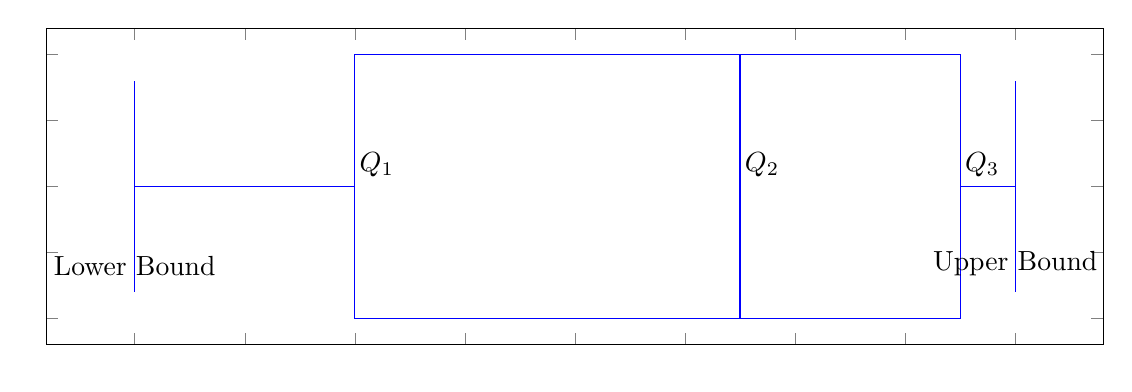
\begin{tikzpicture}
  \begin{axis}
    [
    yticklabels={},
    xticklabels={},
    width=15cm,height=5.6cm,
    ]
    \addplot+[
    boxplot prepared={
      median=98.5,
      upper quartile=100.5,
      lower quartile=95,
      upper whisker=101,
      lower whisker=93
    },
    ] coordinates {};
    \draw[draw=none,] (axis cs:-1,0) -- (axis cs:93,0.7) node[above] {Lower Bound};
    \draw[draw=none,] (axis cs:-1,0) -- (axis cs:95.2,1) node[above] {\(Q_1\)};
    \draw[draw=none,] (axis cs:-1,0) -- (axis cs:98.7,1) node[above] {\(Q_2\)};
    \draw[draw=none,] (axis cs:-1,0) -- (axis cs:100.7,1) node [above] {\(Q_3\)};
    \draw[draw=none,] (axis cs:-1,0) -- (axis cs:101,0.7) node[above] {Upper Bound};
    
  \end{axis}
\end{tikzpicture}
\end{center}
Lower Bound \(= Q_1 - 1.5(Q_3 - Q_1)\)\\
Upper Bound \(= Q_3 + 1.5(Q_3 - Q_1)\)\\
If a value isn't within these boundaries, it's classified as an outlier.
\newpage
\section{Two Variable Statistics}

\begin{center}
    \begin{tikzpicture}
\begin{axis}[
ticks= none,
xmin = 160,xmax = 200,
ymax = 100,
width=15cm,
height=8.5cm,
]
\addplot+[
    only marks,
    scatter,
    mark size=2.9pt]
table[meta]
{data_male.txt};
]
\addplot[domain = 160:210, 
samples=100,
color=black,] {0.53171*x - 13.02362};

%ŷ = 0.53171X - 13.02362
\end{axis}
\end{tikzpicture}
\end{center}
linear correlation (Pearson's R): \(r = \frac{n\displaystyle\sum\limits_{i=1}^{N}x_i y_i - (\displaystyle\sum\limits_{i=1}^{N} x_i)(\displaystyle\sum\limits_{i=1}^{N}y_i)}
{\sqrt{[(n\displaystyle\sum\limits_{i=1}^{N}x_i^2) - (\displaystyle\sum\limits_{i=1}^{N}x_i)^2][(n\displaystyle\sum\limits_{i=1}^{N}y_i^2) - (\displaystyle\sum\limits_{i=1}^{N}y_i)^2]}}\)\\

\begin{center}
    \begin{tabular}{c|c|c}
    Pearson's R value & Strength & Direction\\
    \hline
    \(r > \frac{2}{3}\) & Strong & Positive\\
    \(\frac{1}{3} < r < \frac{2}{3}\) & Moderate & Positive\\
    \(0 < r < \frac{1}{3}\) & Weak & Positive\\
    \(0 & None & None\)\\
    \(-\frac{1}{3} < r < 0\) & Weak & Negative\\
    \(-\frac{2}{3} < r < \frac{1}{3}\) & Moderate & Negative\\
    \(r < -\frac{2}{3} & Strong & Negative\)\\
\end{tabular}
\end{center}

Line of Best Fit \(y = ax+b\): \(a = \frac{n\displaystyle\sum\limits_{i=1}^{N}x_i y_i - (\displaystyle\sum\limits_{i=1}^{N} x_i)(\displaystyle\sum\limits_{i=1}^{N}y_i)}
{n(\displaystyle\sum\limits_{i=1}^{N}x_i^2) - (\displaystyle\sum\limits_{i=1}^{N}x_i)^2}\),\(b = \Bar{y}-a\Bar{x}\), \(\Bar{y} = \frac{\Sigma y}{n}\),\(\Bar{x} = \frac{\Sigma x}{n}\)
\section{Terms}
\begin{itemize}
    \item Cause-and-Effect Relationship: Change in X produces change in Y
    \item Common Cause Factor: External variables cause two variables to change in some way
    \item Accidental Relationship: Correlation exists without any causual relationship
    \item Presumed Relationship: Correlation seems logical with no causual relationships
\end{itemize}
\end{document}
